\documentclass[10pt]{article}
\usepackage[letterpaper,margin=0.9in]{geometry}
\usepackage{amsmath,booktabs,graphicx,float}
\setlength{\parindent}{0pt}\setlength{\parskip}{4pt}
\makeatletter\renewcommand\section{\@startsection{section}{1}{0pt}{-8pt}{3pt}{\normalfont\large\bfseries}}\makeatother
\begin{document}
{\centering\large\textbf{Addendum: $R^2$ scans over Chris's parameters}\par\normalsize 26 September 2026\par}

\section{Method}
The model is column BH of the tab \emph{Copy of Copy of Copy of density}. It is computed with the sheet's formulas unchanged ($\mathsf T=\mathsf R+\mathsf K\,dt$, $dt=1$, $G=6.67\times10^{-17}$, $R=1.3\times10^{23}$\,km, $k=2.18\times10^{-18}$\,s$^{-1}$). The code reproduces the cached BH to $1.6\times10^{-7}$. The fit quality is
\begin{equation}
R^2=1-\frac{\sum_i(y_i-\mathrm{BH}_i)^2}{\sum_i(y_i-\bar y)^2},
\end{equation}
with no refit of slope or offset. Three targets are used: the 71 Migkas points at $\theta=\ell$; $A_F(\ell)$ on a $1^\circ$ grid; and, as a secondary target, the sheet's own lookup-mapped Migkas column AG. The optimiser is a 400-point random screen followed by 25 Nelder--Mead starts. Bounds are $1.05\le D/R\le10$, $0.02\le L/D\le3$, $0.1\le M/M_{\rm sheet}\le10$, $|{\rm BA57}|\le0.15$, and phase in $[0,2\pi)$. None of the best fits lies on a bound.

\textbf{Independent combinations.} BH depends on $D/R$, $L/D$, BA57, BA59 and
\begin{equation}
\Gamma\equiv\frac{G\,M\,dt}{D^2\,k\,R}\qquad(\text{sheet: }0.247).
\end{equation}
$G$, $dt$, $k$ and $R$ enter only through $\Gamma$. Scaling $k$ by $s$ is identical to scaling $M$ by $1/s$, which was checked to machine precision. So $k$ is not scanned separately, and $M$ stands for the gravity strength. Changing the sign of BA57 and adding $\pi$ to BA59 gives the same curve; the tables quote the form with BA57 $<0$.

The optional offset $\ell_0$ sets $\theta=\ell-\ell_0$ and is \emph{not} in the sheet, where $\theta=0$ corresponds to $\ell=0$.

\section{Best fits}
\begin{table}[H]\centering\small\setlength{\tabcolsep}{4pt}
\begin{tabular}{@{}lccccccc|ccc@{}}\toprule
Case & C23 & D23 & B27 $M$ (kg) & BA57 & BA59 (rad) & $\ell_0$ & $\Gamma$ & $R^2_{\rm Migkas}$ & $R^2_{A_F}$ & $R^2_{\rm sheet\,map}$\\\midrule
Sheet values & 5 & 0.18 & $4.44\times10^{68}$ & $-0.06$ & 0.35 & -- & 0.247 & 0.632 & 0.691 & 0.706\\
Best vs Migkas & 2.26 & 0.295 & $6.33\times10^{67}$ & $-0.047$ & 0.21 & -- & 0.173 & \textbf{0.759} & 0.833 & 0.579\\
Best vs $A_F$ & 2.10 & 0.291 & $5.08\times10^{67}$ & $-0.046$ & 0.16 & -- & 0.161 & 0.759 & \textbf{0.834} & 0.573\\
Best vs sheet map & 3.59 & 0.069 & $1.48\times10^{68}$ & $-0.060$ & 0.83 & -- & 0.160 & 0.588 & 0.641 & \textbf{0.790}\\\midrule
\multicolumn{11}{@{}l}{\emph{Optional, with axis offset $\ell_0$ (not in the sheet):}}\\
Best vs Migkas & 2.45 & 0.297 & $9.05\times10^{67}$ & $-0.042$ & 0.45 & $13.0^\circ$ & 0.210 & \textbf{0.897} & 0.981 & --\\
Best vs $A_F$ & 2.32 & 0.295 & $7.69\times10^{67}$ & $-0.041$ & 0.41 & $12.9^\circ$ & 0.199 & 0.896 & \textbf{0.982} & --\\\bottomrule
\end{tabular}\end{table}
For reference, $A_F$ itself scores $R^2=0.915$ against the 71 points.

\section{Profiles}
Figure~\ref{fig:prof} shows $R^2$ against the Migkas points ($\theta=\ell$) for each parameter. One curve holds the other parameters at the sheet values; the other re-optimises them.

\begin{table}[H]\centering\small
\begin{tabular}{@{}lccccc@{}}\toprule
Cell & Sheet & Best & Range with $R^2\ge R^2_{\max}-0.01$ & \multicolumn{2}{c}{Others at sheet values: best value, $R^2$}\\\midrule
C23 $D/R$ & 5 & 2.26 & 1.97--3.12 & 5.18 & 0.636\\
D23 $L/D$ & 0.18 & 0.295 & 0.26--0.30 & 0.26 & 0.680\\
B27 $M$ (kg) & $4.44\times10^{68}$ & $6.3\times10^{67}$ & $\le4.4\times10^{67}$ (bound) -- $1.6\times10^{68}$ & $4.2\times10^{68}$ & 0.637\\
BA57 & $-0.06$ & $-0.047$ & $-0.053$ -- $-0.038$ & $-0.053$ & 0.638\\
BA59 (rad) & 0.35 & 0.21 & $-0.1$ -- 0.47 & 0.63 & 0.656\\
$\ell_0$ (optional) & 0 & $13^\circ$ & $10$--$15^\circ$ & $10^\circ$ & 0.715\\\bottomrule
\end{tabular}\end{table}

\begin{figure}[H]\centering
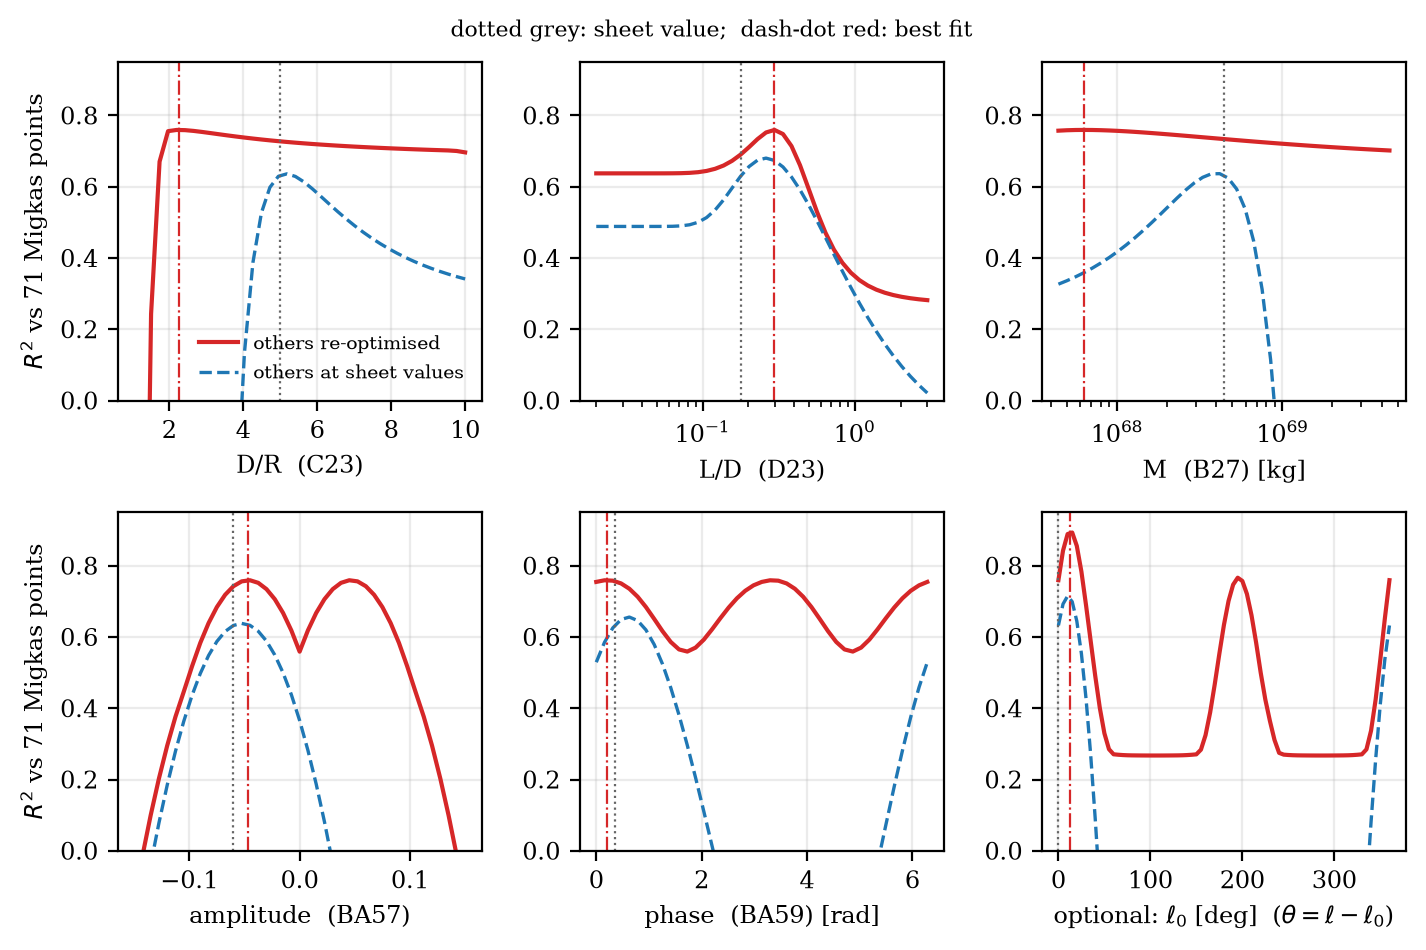
\includegraphics[width=0.92\linewidth]{param_scan_profiles.png}
\caption{$R^2$ profiles against the Migkas points. Solid: others re-optimised. Dashed: others at sheet values. The last panel is the optional $\ell_0$.}\label{fig:prof}
\end{figure}

\begin{figure}[H]\centering
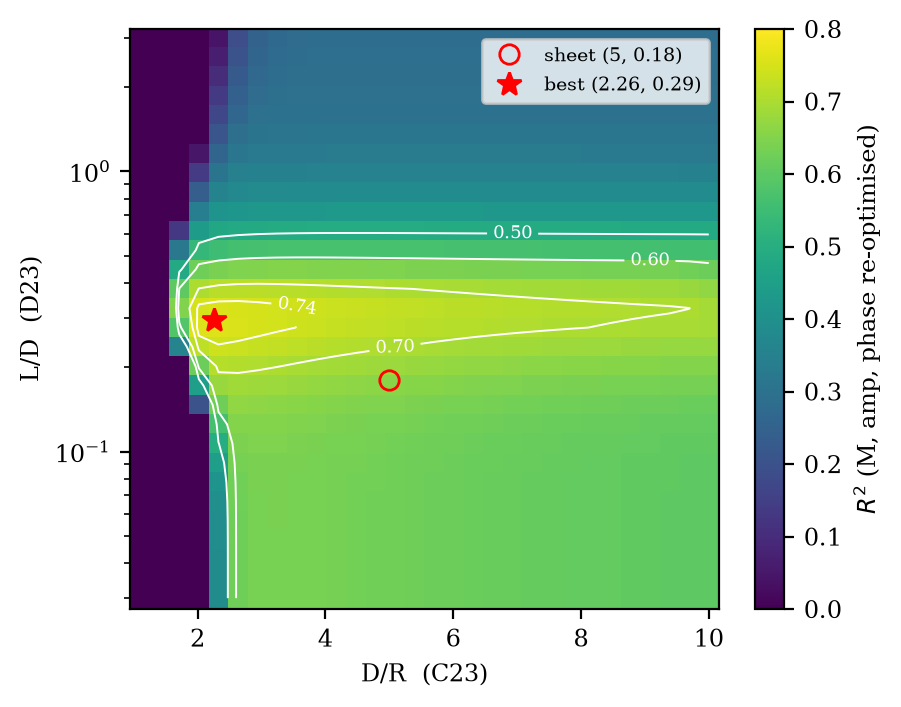
\includegraphics[width=0.56\linewidth]{param_scan_DR_LD.png}
\caption{$R^2$ over $D/R$ and $L/D$, with $M$, BA57 and BA59 re-optimised ($\theta=\ell$).}
\end{figure}

\begin{figure}[H]\centering
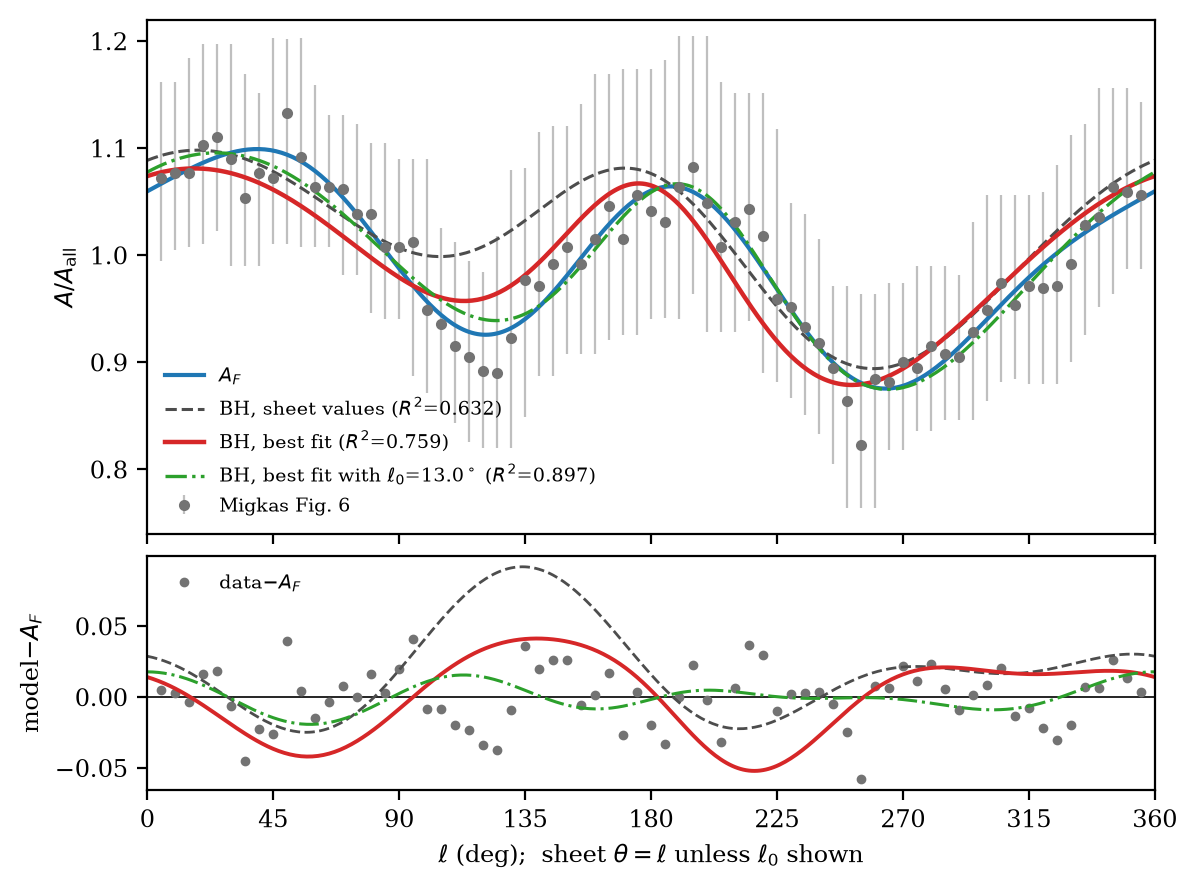
\includegraphics[width=0.8\linewidth]{param_scan_bestfit.png}
\caption{BH at the sheet values, at the best fit, and at the best fit with $\ell_0$, compared with $A_F$ and the Migkas points.}
\end{figure}

\section{Notes}
\begin{enumerate}\setlength{\itemsep}{1pt}
\item $D/R$ and $M$ are strongly degenerate. Along the $D/R$ profile the best $M$ rises roughly as $(D/R)^{3}$ and $R^2$ falls only slowly, from 0.759 to 0.70 at $D/R=10$. Above $D/R\approx9.8$ this re-optimised $M$ reaches the upper bound. Below $D/R\approx1.8$ the fit collapses.
\item $L/D$ is the best-determined parameter (0.26--0.30). The sheet value 0.18 lies outside this range.
\item Without the sine term (BA57 $=0$, geometry re-optimised) the best $R^2$ is 0.559, so the sine term adds 0.20.
\item The largest single gain is the optional $\ell_0\approx13^\circ$, which raises $R^2$ from 0.759 to 0.897 against the points and to 0.98 against $A_F$. The profile has a second, lower peak near $\ell_0\approx195^\circ$ ($R^2\approx0.77$).
\item Fitting the sheet's own lookup mapping favours different geometry ($L/D=0.07$). Its best fits score only 0.59 against the points at $\theta=\ell$.
\end{enumerate}

\sloppy\footnotesize Files in \texttt{papers/spreadsheet\_model/}: \texttt{param\_scan\_core.py}, \texttt{param\_scan.py}, \texttt{param\_scan\_profiles.py}, \texttt{param\_scan\_plots.py}, \texttt{param\_scan\_results.json}, \texttt{param\_scan\_profiles.json}, \texttt{param\_scan\_map.npz}.
\end{document}
